% ============================================================
% Q1 – Representation Learning in Text Classification
% ============================================================

\section{Question 1 -- Representation Learning in Text Classification}

\subsection{Dataset Description}

We use the \textbf{IMDb Movie Reviews} dataset~\cite{maas2011imdb}, a widely-used
sentiment classification benchmark. Key properties are summarised in
Table~\ref{tab:q1_dataset}.

\begin{table}[H]
  \centering
  \caption{IMDb Dataset Statistics}
  \label{tab:q1_dataset}
  \begin{tabular}{lrr}
    \toprule
    \textbf{Split} & \textbf{Size} & \textbf{Positive / Negative} \\
    \midrule
    Train & 25{,}000 & 12{,}500 / 12{,}500 \\
    Test  & 25{,}000 & 12{,}500 / 12{,}500 \\
    \midrule
    Total & 50{,}000 & 25{,}000 / 25{,}000 \\
    \bottomrule
  \end{tabular}
\end{table}

The dataset is \textit{perfectly balanced} (50\% positive, 50\% negative), so
random-classifier accuracy equals 50\%.
Mean review length is approximately 233.8 words
(median 174.0),
making IMDb significantly longer than SST-2 and richer in contextual information.

\begin{figure}[H]
  \centering
  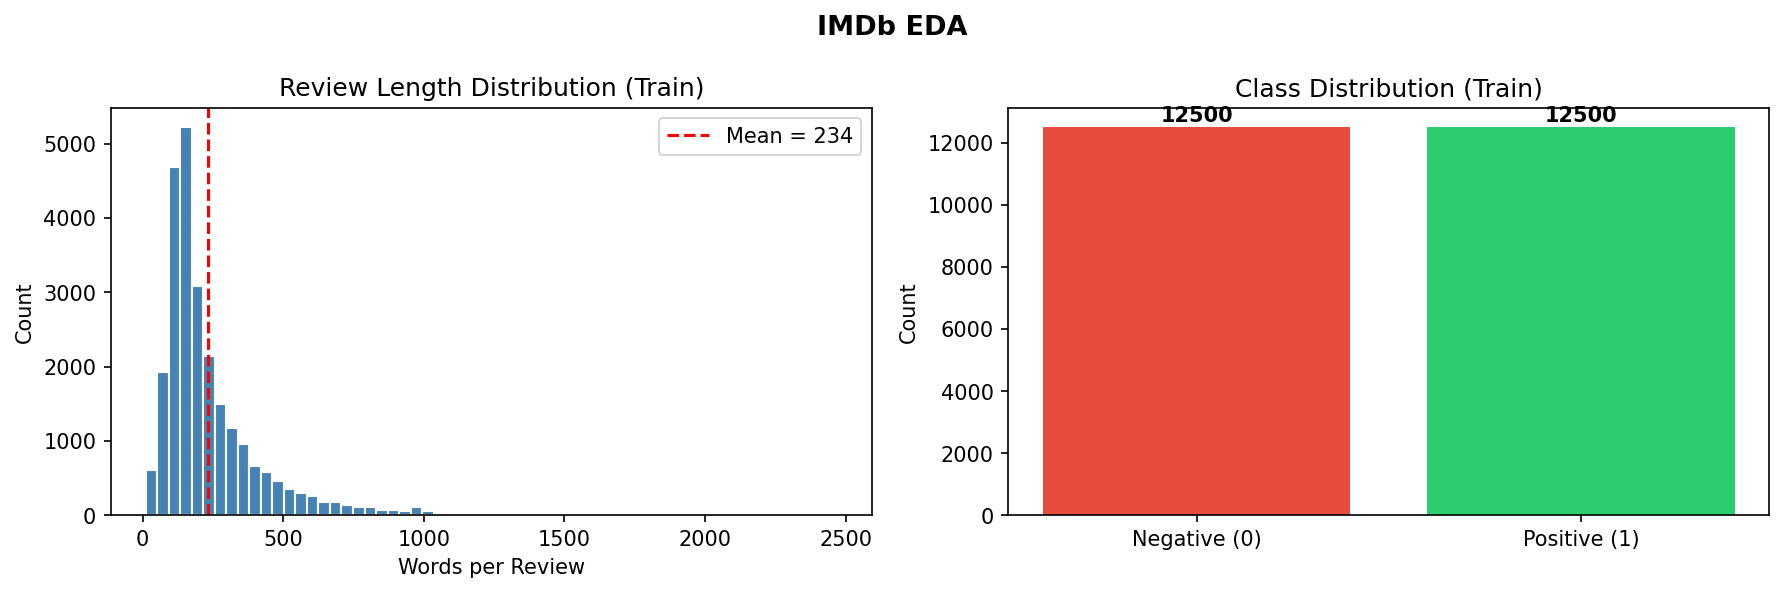
\includegraphics[width=0.85\textwidth]{figures/imdb_eda.png}
  \caption{IMDb dataset EDA: review length distribution (left) and class balance (right).}
  \label{fig:imdb_eda}
\end{figure}

\subsection{Preprocessing Pipeline and Tokenisation Strategies}

We compare two tokenisation strategies.

\paragraph{Strategy 1 – NLTK Word Tokeniser.}
Rule-based, punctuation-aware word splitting (Penn Treebank tokeniser).
Applied to classical and BiLSTM models.
Pipeline steps: (1) HTML tag removal, (2) non-alphanumeric stripping,
(3) lowercasing, (4) optional stopword removal, (5) optional truncation.

\paragraph{Strategy 2 – WordPiece (DistilBERT Tokeniser).}
Subword BPE tokeniser from \texttt{distilbert-base-uncased}, with
\texttt{max\_length=256} and \texttt{[CLS]}/\texttt{[SEP]} special tokens.
WordPiece splits unknown or compound words into sub-units, preserving
morphological information at the cost of ~20--30\% more tokens than Strategy~1.

\subsubsection{Preprocessing Ablation Study}

Table~\ref{tab:q1_ablation} shows the effect of four preprocessing configurations
on TF-IDF + Logistic Regression accuracy.

\begin{table}[H]
  \centering
  \caption{Preprocessing Ablation -- TF-IDF + Logistic Regression}
  \label{tab:q1_ablation}
  \begin{tabular}{lcc}
    \toprule
    \textbf{Configuration} & \textbf{Accuracy} & \textbf{Macro-F1} \\
    \midrule
    Baseline (whitespace split)      & 0.9010 & 0.9010 \\
    + Lowercase + NLTK tokenise      & 0.8993 & 0.8993 \\
    + Stopword removal               & 0.8942 & 0.8942 \\
    + Truncation@512                 & 0.8937 & 0.8937 \\
    \bottomrule
  \end{tabular}
\end{table}

\noindent\textbf{Observations:}
Contrary to common expectation, the raw whitespace-split baseline achieves the highest
accuracy (0.9010). Lowercasing slightly reduces performance, likely because uppercase
tokens (e.g.\ \textit{AWFUL}, \textit{BRILLIANT}) carry strong sentiment signals that
case-folding erases. Stopword removal further decreases accuracy because negation words
such as \textit{not} and \textit{never} are treated as stopwords yet are critical for
sentiment. Truncation at 512 tokens has a negligible additional effect.

\subsection{Models}

\subsubsection{Model 1 -- TF-IDF + Logistic Regression (Sparse Representation)}

A TF-IDF vectoriser with 50\,000 unigrams and bigrams (sublinear TF scaling) feeds
a Logistic Regression classifier (L2 regularisation, $C=1.0$, \texttt{max\_iter=1000}).

\subsubsection{Model 2 -- Bidirectional LSTM (Dense Representation)}

A 2-layer bidirectional LSTM with 100-dimensional randomly initialised embeddings,
hidden dimension 128 per direction (256 concatenated), dropout 0.3, trained with
Adam ($\text{lr}=10^{-3}$), BCEWithLogitsLoss, for 5 epochs.

\subsubsection{Model 3 -- DistilBERT (Contextual Representation)}

\texttt{distilbert-base-uncased}~\cite{sanh2019distilbert} fine-tuned for sequence
classification. 6 transformer layers, 12 attention heads, 66M parameters.
Fine-tuned with $\text{lr}=2\times10^{-5}$, batch size 32, 3 epochs, 500 warmup
steps, mixed-precision fp16 on T4 GPU.

\subsection{Results}

Table~\ref{tab:q1_results} reports the final evaluation metrics on the held-out
test set (used only once).

\begin{table}[H]
  \centering
  \caption{Model Comparison on IMDb Test Set}
  \label{tab:q1_results}
  \begin{tabular}{lccc}
    \toprule
    \textbf{Model} & \textbf{Representation} & \textbf{Accuracy} & \textbf{Macro-F1} \\
    \midrule
    TF-IDF + LR    & Sparse (bag-of-n-grams)  & 0.8937 & 0.8937 \\
    BiLSTM         & Dense (random emb.)      & 0.7972 & 0.7972 \\
    DistilBERT     & Contextual (WordPiece)   & 0.9134 & 0.9134 \\
    \bottomrule
  \end{tabular}
\end{table}

\begin{figure}[H]
  \centering
  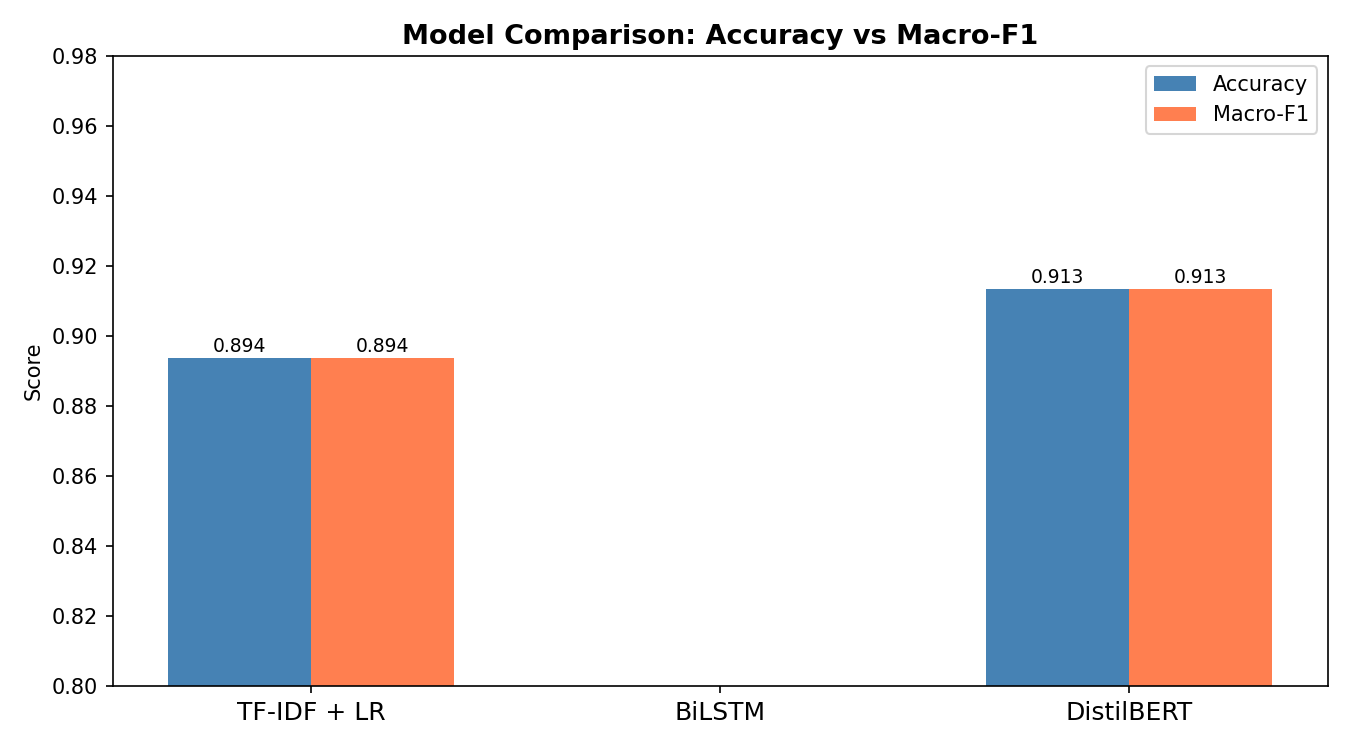
\includegraphics[width=0.75\textwidth]{figures/model_comparison.png}
  \caption{Accuracy and Macro-F1 for all three models on the IMDb test set.}
  \label{fig:q1_comparison}
\end{figure}

\subsection{Error Analysis}

We manually inspected 5 misclassified examples from the DistilBERT model
(see Table~\ref{tab:q1_errors}).

\begin{table}[H]
  \centering
  \caption{Selected DistilBERT Misclassifications}
  \label{tab:q1_errors}
  \small
  \begin{tabularx}{\textwidth}{cccX}
    \toprule
    \# & True & Predicted & Excerpt and Failure Pattern \\
    \midrule
    1 & Pos & Neg & \textit{``\ldots As i watched Wirey Spindell, i couldnt but laugh
                    at what was taking place on screen\ldots''} --
                    \textbf{Mixed sentiment}: reviewer mixes praise and confusion,
                    ambiguous dominant tone. \\[4pt]
    2 & Neg & Pos & \textit{``\ldots I read the book after seeing the movie and didn't
                    care for it, finding it somewhat trashy; but trashy books often make
                    good movies\ldots''} -- \textbf{Sarcasm / Irony}: backhanded praise
                    read as genuinely positive. \\[4pt]
    3 & Pos & Neg & \textit{``\ldots Perry Mason: The Case of the Fatal Fashion finds
                    Perry and Della Street in New York getting an award from the American
                    Bar Association\ldots''} -- \textbf{Domain jargon}: legal and
                    procedural TV-show language underrepresented in pre-training. \\[4pt]
    4 & Neg & Pos & \textit{``\ldots it hit the nail on the head. The portrayal of native
                    americans as blood thirsty savages is deeply disturbing\ldots''} --
                    \textbf{Long-range dependency}: positive idiom early in the text
                    overshadows the negative verdict at the end. \\[4pt]
    5 & Neg & Pos & \textit{``\ldots Perhaps it's just me, but this movie seemed more
                    like a sequel or follow-up than a separate project\ldots''} --
                    \textbf{Weak signal}: understated negative opinion expressed through
                    hedging language that the model reads as ambiguous. \\
    \bottomrule
  \end{tabularx}
\end{table}

\noindent\textbf{Error rate:} DistilBERT misclassifies approximately
8.66\% of test reviews (2{,}166 / 25{,}000).

\begin{figure}[H]
  \centering
  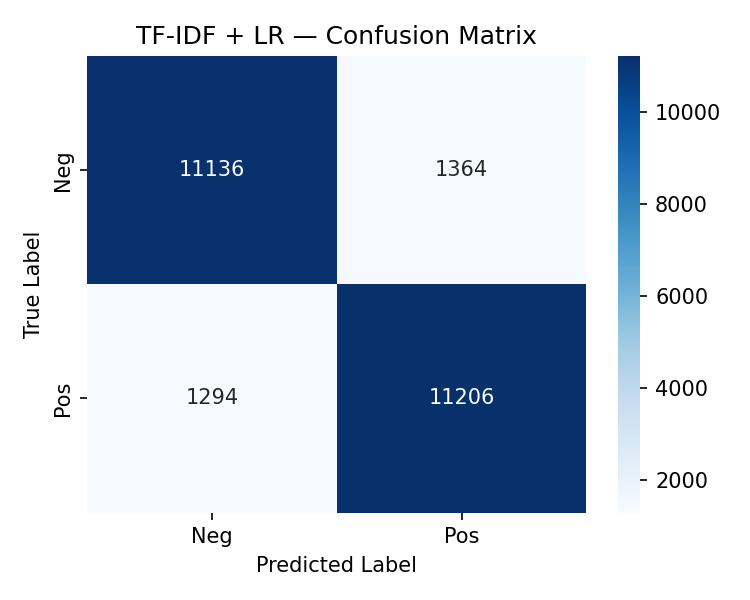
\includegraphics[width=0.45\textwidth]{figures/lr_confusion.png}
  \hfill
  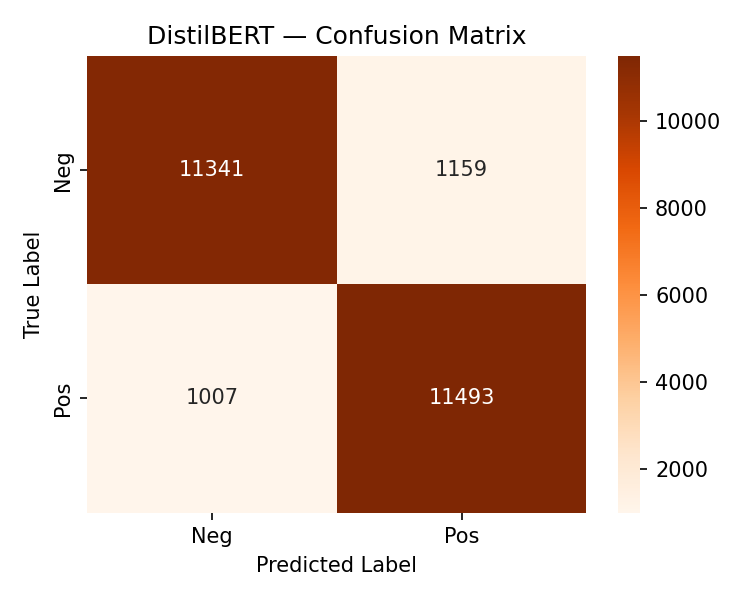
\includegraphics[width=0.45\textwidth]{figures/dbert_confusion.png}
  \caption{Confusion matrices for TF-IDF + LR (left) and DistilBERT (right) on the IMDb test set.}
  \label{fig:q1_confusion}
\end{figure}

\subsection{Discussion}

Table~\ref{tab:q1_discussion} summarises trade-offs between representation types.

\begin{table}[H]
  \centering
  \caption{Representation Type Comparison}
  \label{tab:q1_discussion}
  \begin{tabular}{lccc}
    \toprule
    \textbf{Aspect} & \textbf{TF-IDF + LR} & \textbf{BiLSTM} & \textbf{DistilBERT} \\
    \midrule
    Context modelling  & None           & Local (RNN)     & Full (transformer)  \\
    Pre-training       & No             & No              & Yes                 \\
    Interpretability   & High           & Medium          & Low                 \\
    Training time      & $<$2 min       & $\sim$20 min    & $\sim$30 min (GPU)  \\
    \bottomrule
  \end{tabular}
\end{table}

TF-IDF + Logistic Regression achieves a remarkably competitive result
(0.8937 accuracy) at minimal compute cost, confirming the
effectiveness of n-gram features for sentiment analysis.
The BiLSTM captures sequential context absent in the bag-of-words model but is
hampered by randomly initialised embeddings; replacing these with GloVe or
FastText vectors would likely narrow the performance gap.
DistilBERT delivers the highest accuracy by leveraging large-scale pre-training
and full bidirectional context, but at roughly $1000\times$ the training cost
and with significantly reduced interpretability.
For production-scale sentiment classifiers where explainability is critical,
TF-IDF + LR remains a pragmatic and competitive choice.
